 \section{Les disques protoplanétaires}
%TODO voir thèse mordasini, et les articles de mordasini, alibert, ida et lin, histoire de voir ce qu'ils font)


\subsection{Formation et évolution}
Les planètes se forment à partir d'un disque protoplanétaire constitué de gaz et de poussière. On observe de tels disques autour d'étoiles jeunes, essentiellement pendant les premiers millions d'années de leur existence. Il peut sembler étrange de voir que les disques d'accrétion sont aussi courants dans l'univers et surtout de voir qu'il apparaît spontanément un axe de rotation. 

\begin{figure}[htb]
\centering
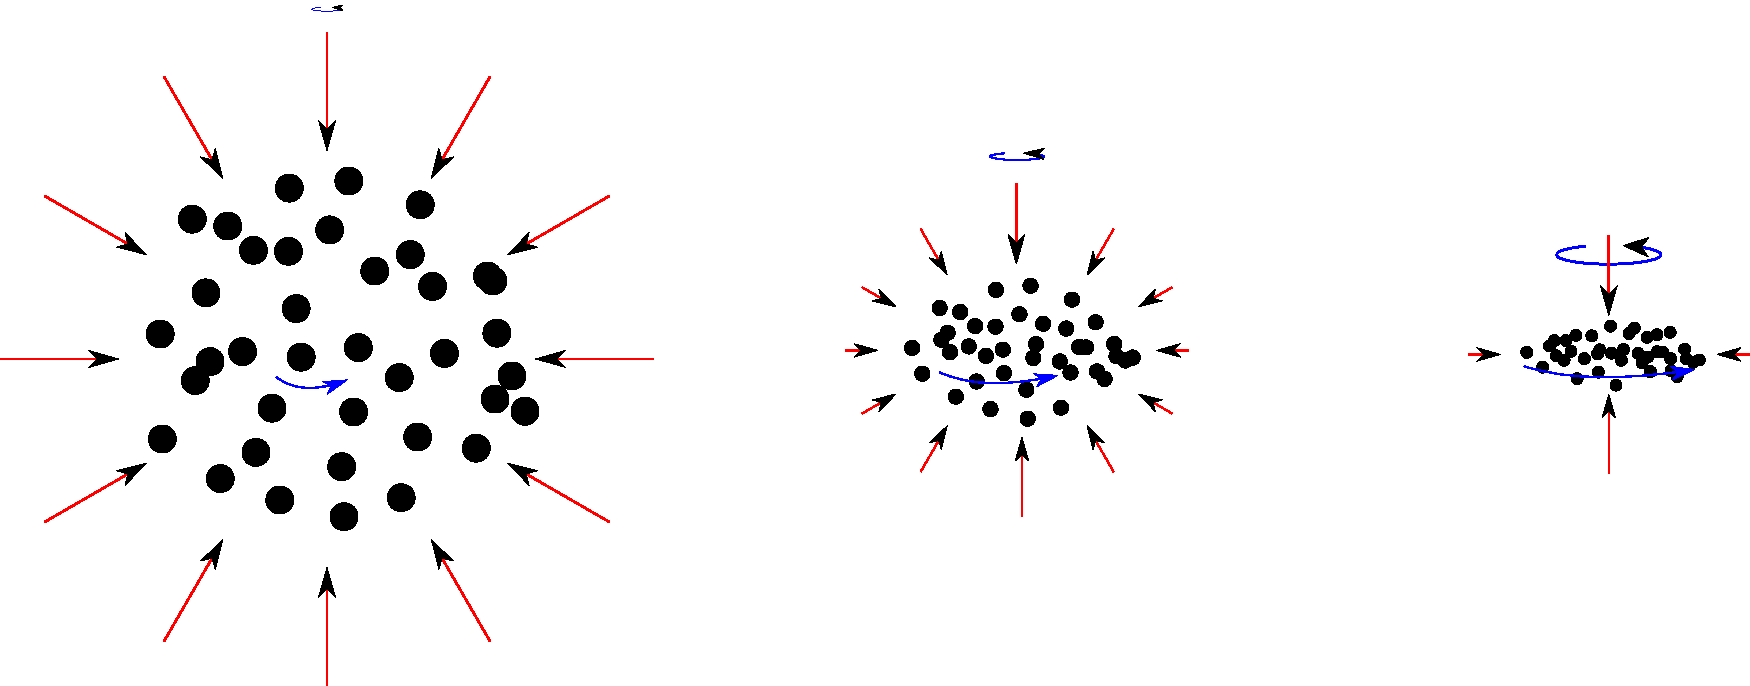
\includegraphics[width=0.8\linewidth]{figure/disk_collapse.pdf}
\caption{Schéma de l'effondrement d'un nuage moléculaire, représenté par un amas épars de cellules de gaz représentées par des points noirs.}\label{fig:disk_collapse}
\end{figure}

\reffig*{fig:disk_collapse} montre le principe de l'effondrement gravitationnel d'un nuage. Loin de moi l'idée de comparer les patineuses avec un nuage de gaz mais pour illustrer l'effondrement gravitationnel d'un nuage moléculaire, rien de mieux que le patinage artistique. 

Quand une patineuse tourne sur elle même, vous observerez qu'en ramenant les bras le long du corps, sa rotation s'accélère. À l'inverse, sa rotation diminue quand elle écarte les bras. C'est une illustration de la conservation du moment angulaire. 

Pour un nuage moléculaire c'est exactement pareil. À mesure que le nuage s'effondre sur lui même, et afin de satisfaire à la conservation du moment angulaire, ce dernier voit sa rotation accélérer. C'est ainsi que le disque d'accrétion, résultat de l'effondrement du nuage de gaz, est en rotation. L'effondrement d'un nuage moléculaire étant beaucoup plus violent que le fait de ramener ses bras le long de son corps, l'accélération de la rotation est elle aussi beaucoup plus drastique dans le cas du nuage. 

Initialement, il est hautement improbable que le moment angulaire du nuage soit parfaitement nul. C'est ainsi que même si sa rotation est imperceptible lors des premiers stades de son effondrement gravitationnel, le disque d'accrétion fini toujours en rotation. 

%\bigskip
%
%L'évolution de tels objets au cours du temps est un sujet de recherche actif, mais le principe de base est que lors de l'effondrement gravitationnel d'un nuage moléculaire diffus, le gigantesque moment angulaire de cette masse ne peut s'évacuer instantanément. 
%
%La quantité totale de moment angulaire doit être conservée. En conséquence, soit deux cellules de gaz vont échanger du moment angulaire par friction (celle qui gagne du moment angulaire migre vers l'extérieur, l'autre migrant vers l'intérieur), soit du moment angulaire est perdu soit par accrétion d'une particule de gaz sur l'étoile, soit par évaporation du gaz sur les bords du disque.
%
%Mais ces processus prennent du temps, beaucoup plus de temps que n'en met le gaz pour faire une orbite autour de l'étoile. De l'ordre du million d'années. C'est durant ce labs de temps que les planètes se forment. Le processus est complexe et très loin d'être compris. Il est cependant clair que les interactions entre le disque de gaz et les planètes ont un rôle prépondérant dans la formation d'un système stellaire, que ce soit pour les planètes géantes, dont on pense qu'elles ont accrété une partie du gaz du disque pour en faire leur enveloppe, ou les planètes telluriques, beaucoup plus denses, principalement composées des poussières du disque.
%
%\bigskip
%
%Afin de décrire la physique des disques, on a besoin principalement de deux équations. L'équation de Navier-Stokes pour décrire le comportement fluide du disque de gaz et l'équation de conservation de l'énergie, pour décrire la température du disque.

\subsection{Évolution hydrodynamique du disque}
Avant de considérer l'évolution d'un disque, il est important de regarder sa masse par rapport à la masse de l'étoile centrale. En effet, si la masse du disque est de l'ordre de la masse de l'étoile, alors des instabilités se développent et on ne peut plus négliger l'autogravité du disque. 

Le \gras{paramètre de Toomre} $Q$, défini par :
\begin{align}
Q &= \frac{\kappa {c_{s}}^2}{\pi G \Sigma}
\end{align}\index{$Q$}
est un indicateur de la stabilité du disque par rapport à l'autogravité.

La densité de surface $\Sigma$\index{$\Sigma$} mesure l'importance de l'\gras{auto-gravité}. La vitesse du son $c_{s}$ est liée à la pression thermique ; la \gras[fréquence!epicyclique@épicyclique]{fréquence épicyclique} $\kappa$ détermine quant à elle la force du cisaillement dans le disque.

\bigskip

Si $Q<1$ alors le gaz est instable gravitationnellement et il commence à s'effondrer sur lui même et former des \og tas\fg de matière.
Si $Q>1$, le disque est stable.

%\begin{remarque}
%Dans les disques protoplanétaires, $Q\gg 1$ ce qui implique que leur auto-gravité n'est pas importante \citep{masset2008planet}.
%\end{remarque}

Nous ne considérerons que des disques dont la masse $M_\text{d}$ est faible devant la masse de l'étoile $M_\star$ :
\begin{align}
\frac{M_\text{d}}{M_\star} &\lesssim 0.1
\end{align}
Si tel n'était pas le cas, le temps pour que le disque perde suffisamment de masse pour se retrouver dans le cas qui nous intéresse sera court devant la vie du disque et le temps de formation planétaire. Étant donné qu'on ne s'intéresse qu'aux derniers stades de la formation planétaire, à savoir quand les embryons planétaires ont une masse de l'ordre du dixième de masse terrestre au minimum, il est raisonnable de penser que le disque sera dans un stade peu dense où l'approximation $Q>1$ sera valable.

Dans un tel cas, c'est le potentiel gravitationnel de l'étoile qui domine la dynamique du gaz. En négligeant l'effet de la pression de ce dernier, on peut donc écrire la vitesse angulaire du gaz comme étant égale à la vitesse angulaire képlerienne : 
\begin{align}
\Omega &= \sqrt{\frac{GM_\star}{r^3}}
\end{align}
où $G$ est la constante de gravitation, et $r$ la distance à l'étoile. Dans la pratique, il est à noter que la vitesse est légèrement sous-képlerienne. 

\bigskip

À l'instar des planètes du système solaire qui orbitent autour du Soleil d'autant plus vite qu'elle sont proche de ce dernier, les éléments fluides du disques de gaz vont orbiter beaucoup plus vite au bord interne qu'ils ne le font au bord externe. Il existe donc une force de cisaillement entre deux anneaux de gaz concentriques, dûs à leur différence de vitesse. Cette différence de vitesse génère des frottements à cause de la viscosité du disque $\nu$ (dont nous parlerons plus en détail plus loin \refsec{sec:viscosite}) qui chauffe le gaz en lui faisant perdre de l'énergie. En conséquence, une partie de l'énergie gravitationnelle du gaz est convertie en chaleur, qui est ensuite évacuée par le rayonnement de corps noir du gaz. 

\bigskip

La première conséquence est qu'un terme visqueux va apparaître dans l'équation de l'énergie, comme nous le verrons par la suite. 

La deuxième conséquence, c'est que le gaz perds de l'énergie, et donc dérive lentement vers l'étoile centrale qui accrète petit à petit le gaz du disque. 

On définit donc une vitesse de dérive négative $\vect{v_d} = v_r \hat{e}_r$, orientée vers l'étoile, qui entraine petit à petit le gaz du disque (avec $v_r$ négatif).

Dans la suite de la section, nous allons nous intéresser à la conservation de différentes quantités, que ce soit la masse ou le moment angulaire. Pour cela nous allons définir un anneau de référence, portion du disque sur laquelle nous allons faire le bilan. Le but est ici de présenter d'où viennent les équations et plus précisément d'où viennent les termes des équations. 

\bigskip

Afin de décrire l'évolution hydrodynamique du disque de gaz, nous allons utiliser successivement la \textbf{conservation de la masse}, et la \textbf{conservation du moment angulaire.}


\subsubsection{Bilan de masse}
\begin{figure}[htb]
\centering
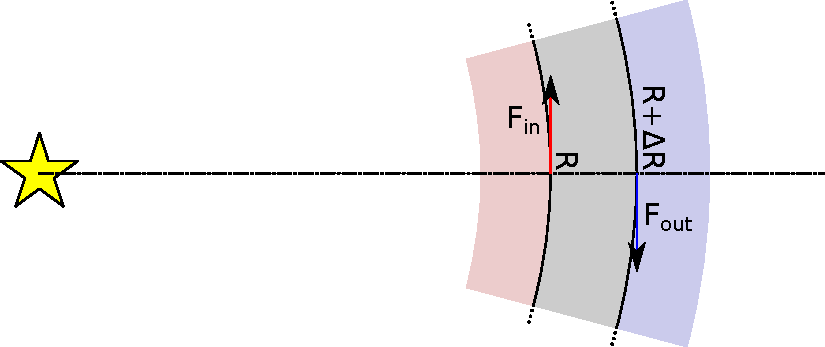
\includegraphics[width=0.7\linewidth]{figure/disk_ring.pdf}
\caption{Représentation d'un anneau de largeur $\Delta r$ et du bilan de moment angulaire de ce dernier.}\label{fig:disk_ring}
\end{figure}

On cherche dans un premier temps à faire le bilan de masse de l'anneau considéré. Sa masse s'écrit :
\begin{align}
m_a &= 2\pi R \Delta R \Sigma(R)\label{eq:m_a}
\end{align}

\bigskip

Soit $v_r\hat{e}_r$ la vitesse radiale du gaz (avec $v_r<0$ dans notre cas). Cette vitesse est responsable d'un certain taux d'accrétion du gaz du disque sur l'étoile centrale. On cherche maintenant à modéliser cette accrétion pour le bilan de moment cinétique sur l'anneau.

Pour cela, on cherche à exprimer la variation de masse de l'anneau, ainsi que le moment cinétique emporté par cette variation de masse. 

Au bord interne $R$, par unité de temps, la masse entrant ou sortant de l'anneau peut-être exprimée comme un flux :
\begin{align}
\dif F_M &= \Sigma \cdot 2\pi r \cdot \left( -\vect{v_r} \cdot \vect{\dif S} \right)
\end{align}
En effet, en multipliant la circonférence de l'anneau par la vitesse, on obtient une sorte de surface par unité de temps qui représente ce qui sort de la frontière virtuelle représentée par l'anneau en $r=R$. 

On note aussi qu'on effectue le produit scalaire entre $\vect{\dif S}$, le vecteur élément de surface, orienté vers l'extérieur de l'anneau et la vitesse. Un signe moins est appliqué, car si le vecteur vitesse et l'élément de surface sont colinéaires, alors la masse sort de l'anneau, c'est donc un flux négatif.

On a ainsi aux deux bords de l'anneau :
\begin{subequations}
\begin{align}
\dif F_M(R) &= \Sigma(R) \cdot 2\pi R \cdot v_r(R)\\
\dif F_M(R+\Delta R) &= - 2\pi (R+\Delta R) \cdot v_r(R+\Delta R) \cdot \Sigma(R+\Delta R)
\end{align}\label{eq:dif_F_M}
\end{subequations}
$v_r$ étant négatif, on a bien une perte de masse en $r=R$ et un gain de masse en $r=R+\Delta R$.

La conservation de la masse implique alors que la dérivée temporelle de la masse de l'anneau est égale au flux de masse à travers sa surface. On a ainsi : 
\begin{align*}
\dpd{}{t}\left(2\pi R \Delta R \Sigma(R)\right) &= \dif F_M(R) + \dif F_M(R+\Delta R)\\
\dpd{}{t}\left(\cancel{2\pi}R \Delta R \Sigma(R)\right) &= \Sigma(R) \cdot \cancel{2\pi} R \cdot v_r(R) - \cancel{2\pi} (R+\Delta R) \cdot v_r(R+\Delta R) \cdot \Sigma(R+\Delta R)
\end{align*}

$R$ et $\Delta R$ sont des variables indépendantes du temps. On peut donc les sortir de la dérivée partielle en fonction du temps. 

En faisant passer le terme $\Delta R$ dans le second membre de l'équation, on fait apparaître des termes de la forme 
\begin{align*}
\frac{U(R+\Delta R) - U(R)}{\Delta R}
\end{align*}

En faisant tendre l'épaisseur $\Delta R$ de l'anneau vers 0, on fait ainsi apparaitre une forme différentielle : 
\begin{align*}
\lim_{\Delta R \rightarrow 0} \frac{U(R+\Delta R) - U(R)}{\Delta R} &= \dpd{U}{r}(R)
\end{align*}

On obtient alors :
\begin{important}
\begin{align}
\dpd{\Sigma}{t} + \inv{R}\dpd{}{r}\left(R v_r \Sigma\right)&=0\label{eq:conservation_masse}
\end{align}
\end{important}

\subsubsection{Bilan de moment cinétique/angulaire}
On cherche maintenant à faire le bilan de moment cinétique de ce même anneau. Son moment cinétique est défini par :
\begin{align}
\vect{J_a} &= \vect{R} \wedge (m_a\vect{v(R)}) \nonumber\\
&= m_a \cdot R \cdot R\Omega(R)\nonumber\\
&= 2\pi R \Delta R \Sigma(R)\cdot R \cdot R\Omega(R)\nonumber\\
\vect{J_a} &= 2\pi R^3 \Delta R \Sigma(R)\Omega(R)\label{eq:J_a}
\end{align}
où $\Sigma$ et $\Omega$ sont la densité de surface et la vitesse angulaire du gaz à la position $R$ dans le disque.

Le flux de moment cinétique est simplement défini comme la quantité de moment cinétique emportée ou apportée par le flux de masse définis précédemment \refeq{eq:dif_F_M} :
\begin{subequations}
\begin{align}
\dif J(R) &= \vect{r} \wedge \left(\dif F_M(R) \vect{v}(R)\right)\nonumber\\
 &= \dif F_M(R) \cdot R^2\Omega(R)\hat{e}_z\nonumber\\
\dif J(R) &= 2\pi v_r(R) \Sigma(R)\cdot R^3\Omega(R)\hat{e}_z\label{eq:dJ_in}\\
\dif J(R+\Delta R) &= \vect{r} \wedge \left(\dif M(R+\Delta R) \vect{v}(R+\Delta R)\right)\nonumber\\
 &= \dif F_M(R+\Delta R) \cdot \left(R+\Delta R\right)^2\Omega(R+\Delta R)\hat{e}_z\nonumber\\
\dif J(R+\Delta R) &= 2\pi v_r(R+\Delta R) \Sigma(R+\Delta R)\cdot \left(R+\Delta R\right)^3\Omega(R+\Delta R)\hat{e}_z\label{eq:dJ_out}
\end{align}\label{eq:dJ}
\end{subequations}

\bigskip

À ceci s'ajoute la variation de moment cinétique induite par la friction entre anneaux concentriques, en d'autres termes, dus à la viscosité du disque. Cette variation de moment cinétique est représentée sous la forme d'un couple exercé par les anneaux internes et externes à celui considéré. 

Le taux de cisaillement $A$ est donné par : 
\begin{align}
A &= r \dod{\Omega}{r}
\end{align}
et est une illustration de la viscosité d'un fluide. Plus le fluide est visqueux, et moins le cisaillement est important. C'est à dire que plus un fluide est visqueux, et plus son comportement se rapproche de celui d'un solide. En conséquence, par frottement, les éléments fluides sont agglomérés, et le gradient de vitesse est très faible, le cisaillement l'est aussi par extension. 

La force visqueuse par unité de longueur est définie par :
\begin{align}
\dif F_\text{vis} &= \nu \Sigma A = \nu \Sigma r \dod{\Omega}{r}
\end{align}

La force visqueuse induite par les anneaux entourant l'anneau considéré est alors : 
\begin{subequations}
\begin{align}
\vect{F_\text{in}}(R) &= 2\pi R \times \dif F_\text{vis}(R) \nonumber\\
\vect{F_\text{in}}(R)&= 2\pi\nu \Sigma R^2 \dod{\Omega}{r}(R) \hat{e}_\theta\\
\vect{F_\text{out}}(R+\Delta R) &= 2\pi (R+\Delta R) \times \dif F_\text{vis}(R+\Delta R) \nonumber\\
\vect{F_\text{out}}(R+\Delta R)&= 2\pi\nu \Sigma (R+\Delta R)^2 \dod{\Omega}{r}(R+\Delta R) \cdot \hat{e}_\theta
\end{align}
\end{subequations}
L'anneau interne tournant plus vite, la force est dirigée dans le sens de rotation $\hat{e}_\theta$. À l'inverse, l'anneau externe tourne moins vite, il tend à freiner l'anneau de référence et s'oppose à son mouvement. La force est donc opposée au sens de rotation.

\bigskip

Ainsi, le couple $\vect{\Gamma}=\vect{r}\wedge\vect{F}$ issu de chacun des anneaux entourant celui de référence s'écrit :
\begin{subequations}
\begin{align}
\vect{\Gamma_\text{in}} &= R\hat{e}_r\wedge\vect{F_\text{in}}\nonumber\\
\vect{\Gamma_\text{in}} &= 2\pi\nu \Sigma R^3 \dod{\Omega}{r}(R) \hat{e}_z\label{eq:G_in}\\
\vect{\Gamma_\text{out}} &= (R+\Delta R)\hat{e}_r\wedge\vect{F_\text{out}}\nonumber\\
\vect{\Gamma_\text{out}} &= 2\pi\nu \Sigma (R+\Delta R)^3 \dod{\Omega}{r}(R+\Delta R) \hat{e}_z\label{eq:G_out}
\end{align}\label{eq:J_torques}
\end{subequations}

\bigskip

On fait maintenant un bilan des variations de moment angulaire pour l'anneau de gaz. Pour celà on dit que la variation de moment angulaire (que l'on écrit en dérivant $J_a(t)$) est égale aux variations de moment angulaires induites aux bords de l'anneau par échange de masse à laquelle s'ajoute la différence entre les deux couples visqueux qui s'appliquent au bord externe et interne. Ce qui donne : 
\begin{align}
\dod{J_a}{t} &= \dif J(R+\Delta R) + \dif J(R) + \Gamma_\text{out} - \Gamma_\text{in}\label{eq:cons_J_a}
\end{align}

En utilisant \refeq{eq:J_a}, \refeq{eq:dJ}, \refeq{eq:J_torques}, dans \refeq{eq:cons_J_a}
\begin{align*}
\begin{split}
\dpd{}{t}\left(2\pi R^3 \Delta R \Sigma(R)\Omega(R)\right) &= -\left(R+\Delta R\right)^3v_R(R+\Delta R) \Sigma(R+\Delta R) \Omega(R+\Delta R)\\
& + R^3 v_R(R) \Sigma(R) \Omega(R) + \left[\nu(R+\Delta R)^3\Sigma(R+\Delta R)\right.\\
&\left. \dod{\Omega}{r}(R+\Delta R)-\nu \Sigma(R) R^3 \dod{\Omega}{r}(R)\right]
\end{split}
\end{align*}



On fait tendre $\Delta R$ vers 0, et de manière similaire au bilan de masse obtenu précédemment, il vient alors 
\begin{align*}
\dpd{}{t}\left(R^3 \Sigma\Omega\right) &= -\dpd{}{r}\left(R^3 v_R \Sigma \Omega\right) + \dpd{}{r}\left(\nu \Sigma R^3 \dod{\Omega}{r}\right)\\
\intertext{$R$ et $t$ sont des variables indépendantes, on peut donc sortir $R$ de la dérivée partielle temporelle afin de faire apparaître une forme qui fait penser à une équation de continuité.}
R\dpd{}{t}\left(R^2 \Sigma\Omega\right) &= -\dpd{}{r}\left(R^3 v_R \Sigma \Omega\right) + \dpd{}{r}\left(\nu \Sigma R^3 \dod{\Omega}{r}\right)
\end{align*}

$R$ et $t$ étant des variables indépendantes, on peut écrire :
\begin{align}
R\dpd{}{t}\left(\Sigma R^2\Omega\right) + \dpd{}{r}\left(R^3 v_R \Sigma \Omega\right) &= \dpd{}{r}\left(\nu \Sigma R^3 \dod{\Omega}{r}\right)\label{eq:ang_mom_01}
\end{align}

\bigskip

On suppose que $\dpd{\Omega}{t}=0$ vu que le potentiel gravitationnel est indépendant du temps (on ne considère pas une masse variable de l'étoile due à l'accrétion), et sachant que $R$ ne dépend pas explicitement de $t$, en utilisant la formule : 
\begin{align*}
\dpd{uv}{x} &= \dpd{u}{x}v + u\dpd{v}{x}
\end{align*}
on peut écrire :
\begin{align}
\dpd{}{t}\left(\Sigma\cdot R^2\Omega\right) &= \left(R^2\Omega\right)\dpd{\Sigma}{t} + \Sigma\cancelto{0}{\dpd{R^2\Omega}{t}}\label{eq:ang_mom_tmp_01}
\end{align}

De même : 
\begin{align}
\dpd{}{r}\left(R^3 v_R \Sigma \Omega\right) &= \dpd{}{r}\left(R v_R \Sigma \cdot R^2\Omega\right)\nonumber\\
&= \left(R^2\Omega\right)\dpd{}{r}\left(R v_R \Sigma\right) + R \Sigma v_R \dpd{}{r}\left(R^2\Omega\right)\label{eq:ang_mom_tmp_02}
\end{align}

En utilisant \refeq{eq:ang_mom_tmp_01} et \refeq{eq:ang_mom_tmp_02} dans \refeq{eq:ang_mom_01}, on fait alors apparaître \refeq{eq:conservation_masse}, ce qui donne : 
\begin{align}
R\left(R^2\Omega\right)\dpd{\Sigma}{t} + \left(R^2\Omega\right)\dpd{}{r}\left(R v_R \Sigma\right) + R \Sigma v_R \dpd{}{r}\left(R^2\Omega\right) &= \dpd{}{r}\left(\nu \Sigma R^3 \dod{\Omega}{r}\right)\nonumber\\
\left(R^2\Omega\right)\cancelto{0}{\left[R\dpd{\Sigma}{t} + \dpd{}{r}\left(R v_R \Sigma\right)\right]} + R \Sigma v_R \dpd{}{r}\left(R^2\Omega\right) &= \dpd{}{r}\left(\nu \Sigma R^3 \dod{\Omega}{r}\right)\nonumber\\
R \Sigma v_R \dpd{}{r}\left(R^2\Omega\right) &= \dpd{}{r}\left(\nu \Sigma R^3 \dod{\Omega}{r}\right)\nonumber\\
R \Sigma v_R &= \inv{\dpd{}{r}\left(r^2\Omega\right)} \dpd{}{r}\left(\nu \Sigma R^3 \dod{\Omega}{r}\right)\label{eq:r_sigma_vr}
\end{align}

\bigskip

On injecte alors \refeq{eq:r_sigma_vr} dans \refeq{eq:conservation_masse} afin de supprimer $v_r$ de l'expression et obtenir finalement : 
\begin{align*}
\dpd{\Sigma}{t} &= -\inv{r}\dpd{}{r}\left[\inv{\dpd{}{r}\left(R^2\Omega\right)} \dpd{}{r}\left(\nu \Sigma r^3 \dod{\Omega}{r}\right)\right]
\end{align*}

On décale le signe moins au niveau de la dérivée de la vitesse angulaire, cette dernière étant généralement négative, ça permet d'avoir un terme positif :
\begin{important}
\begin{align}
\dpd{\Sigma}{t} &= \inv{r}\dpd{}{r}\left\{\inv{\dpd{}{r}\left(r^2\Omega\right)} \dpd{}{r}\left[\nu \Sigma r^3 \left(-\dod{\Omega}{r}\right)\right]\right\}
\end{align}
\end{important}

\bigskip

On fait maintenant l'approximation que le mouvement est képlérien, avec pour première conséquence que $\Omega = \sqrt{\frac{GM}{r^3}}$. On peut alors simplifier l'équation : 
\begin{align*}
\dpd{\Sigma}{t} &= \inv{r}\dpd{}{r}\left\{\inv{\inv{2}\sqrt{\frac{GM}{r}}} \dpd{}{r}\left[\nu \Sigma r^3 \left(\frac{3}{2}\sqrt{\frac{GM}{r^5}}\right)\right]\right\}\nonumber\\
&= \inv{R}\dpd{}{r}\left\{\bcancel{2}\sqrt{\frac{r}{\cancel{GM}}} \dpd{}{r}\left[\nu \Sigma \frac{3}{\bcancel{2}}\cancel{\sqrt{GM}}r^\sfrac{1}{2}\right]\right\}\nonumber\\
\end{align*}

\subsubsection{Conclusion de la partie}
On obtient alors l'équation suivante : 
\begin{important}
\begin{align}
\dpd{\Sigma}{t} &=\frac{3}{r}\dpd{}{r}\left[\sqrt{r} \dpd{}{r}\left(\nu \Sigma r^\sfrac{1}{2}\right)\right]
\end{align}
\end{important}

Cette équation a nécessité les approximations suivantes : 
\begin{enumerate}
\item On suppose que le potentiel gravitationnel est indépendant du temps ($\dod{\Omega}{t}=0$), c'est à dire que la masse de l'étoile est constante, l'accrétion ayant un effet négligeable.
\item On suppose que le mouvement du gaz est képlerien $\Omega=\sqrt{\frac{GM}{r^3}}$, ce qui n'est pas rigoureusement vrai, la pression du gaz rendant le mouvement légèrement sous-képlerien.
\end{enumerate}

\subsection{Profil de température}
Du point de vue de la température, il y a principalement deux types de disques : 
\begin{itemize}
\item les \gras[disque actif]{disques actifs} : la source de température est le disque lui même, qui par \gras{chauffage visqueux} (frottements) va convertir de l'énergie gravitationnelle en chaleur ;
\item les \gras[disque passif]{disques passifs} : la source de chaleur/température est l'étoile centrale qui éclaire le disque. 
\end{itemize}

Un disque peut à la fois être actif et passif, mais généralement on essaie d'approximer, de considérer que l'un est négligeable devant l'autre. De plus, un disque aura des zones actives et des zones passives, c'est à dire que certaines zones seront principalement chauffées par la viscosité alors que d'autres le seront par l'\gras{irradiation de l'étoile}.

\bigskip

Afin de déterminer le profil de température, il faut écrire l'équation de conservation de l'énergie, qui va tenir compte de tous les termes source et toutes les pertes, par unité de surface.

On a tout d'abord les pertes par rayonnement de corps noir. Ensuite, il y a les termes sources, qui peuvent dépendre en fonction de la physique que l'on considère. Pour notre cas, il y a un terme dû à l'enveloppe du disque, un dû à l'irradiation de l'étoile centrale, et enfin un dernier dû au chauffage visqueux.


\begin{figure}[htb]
\centering
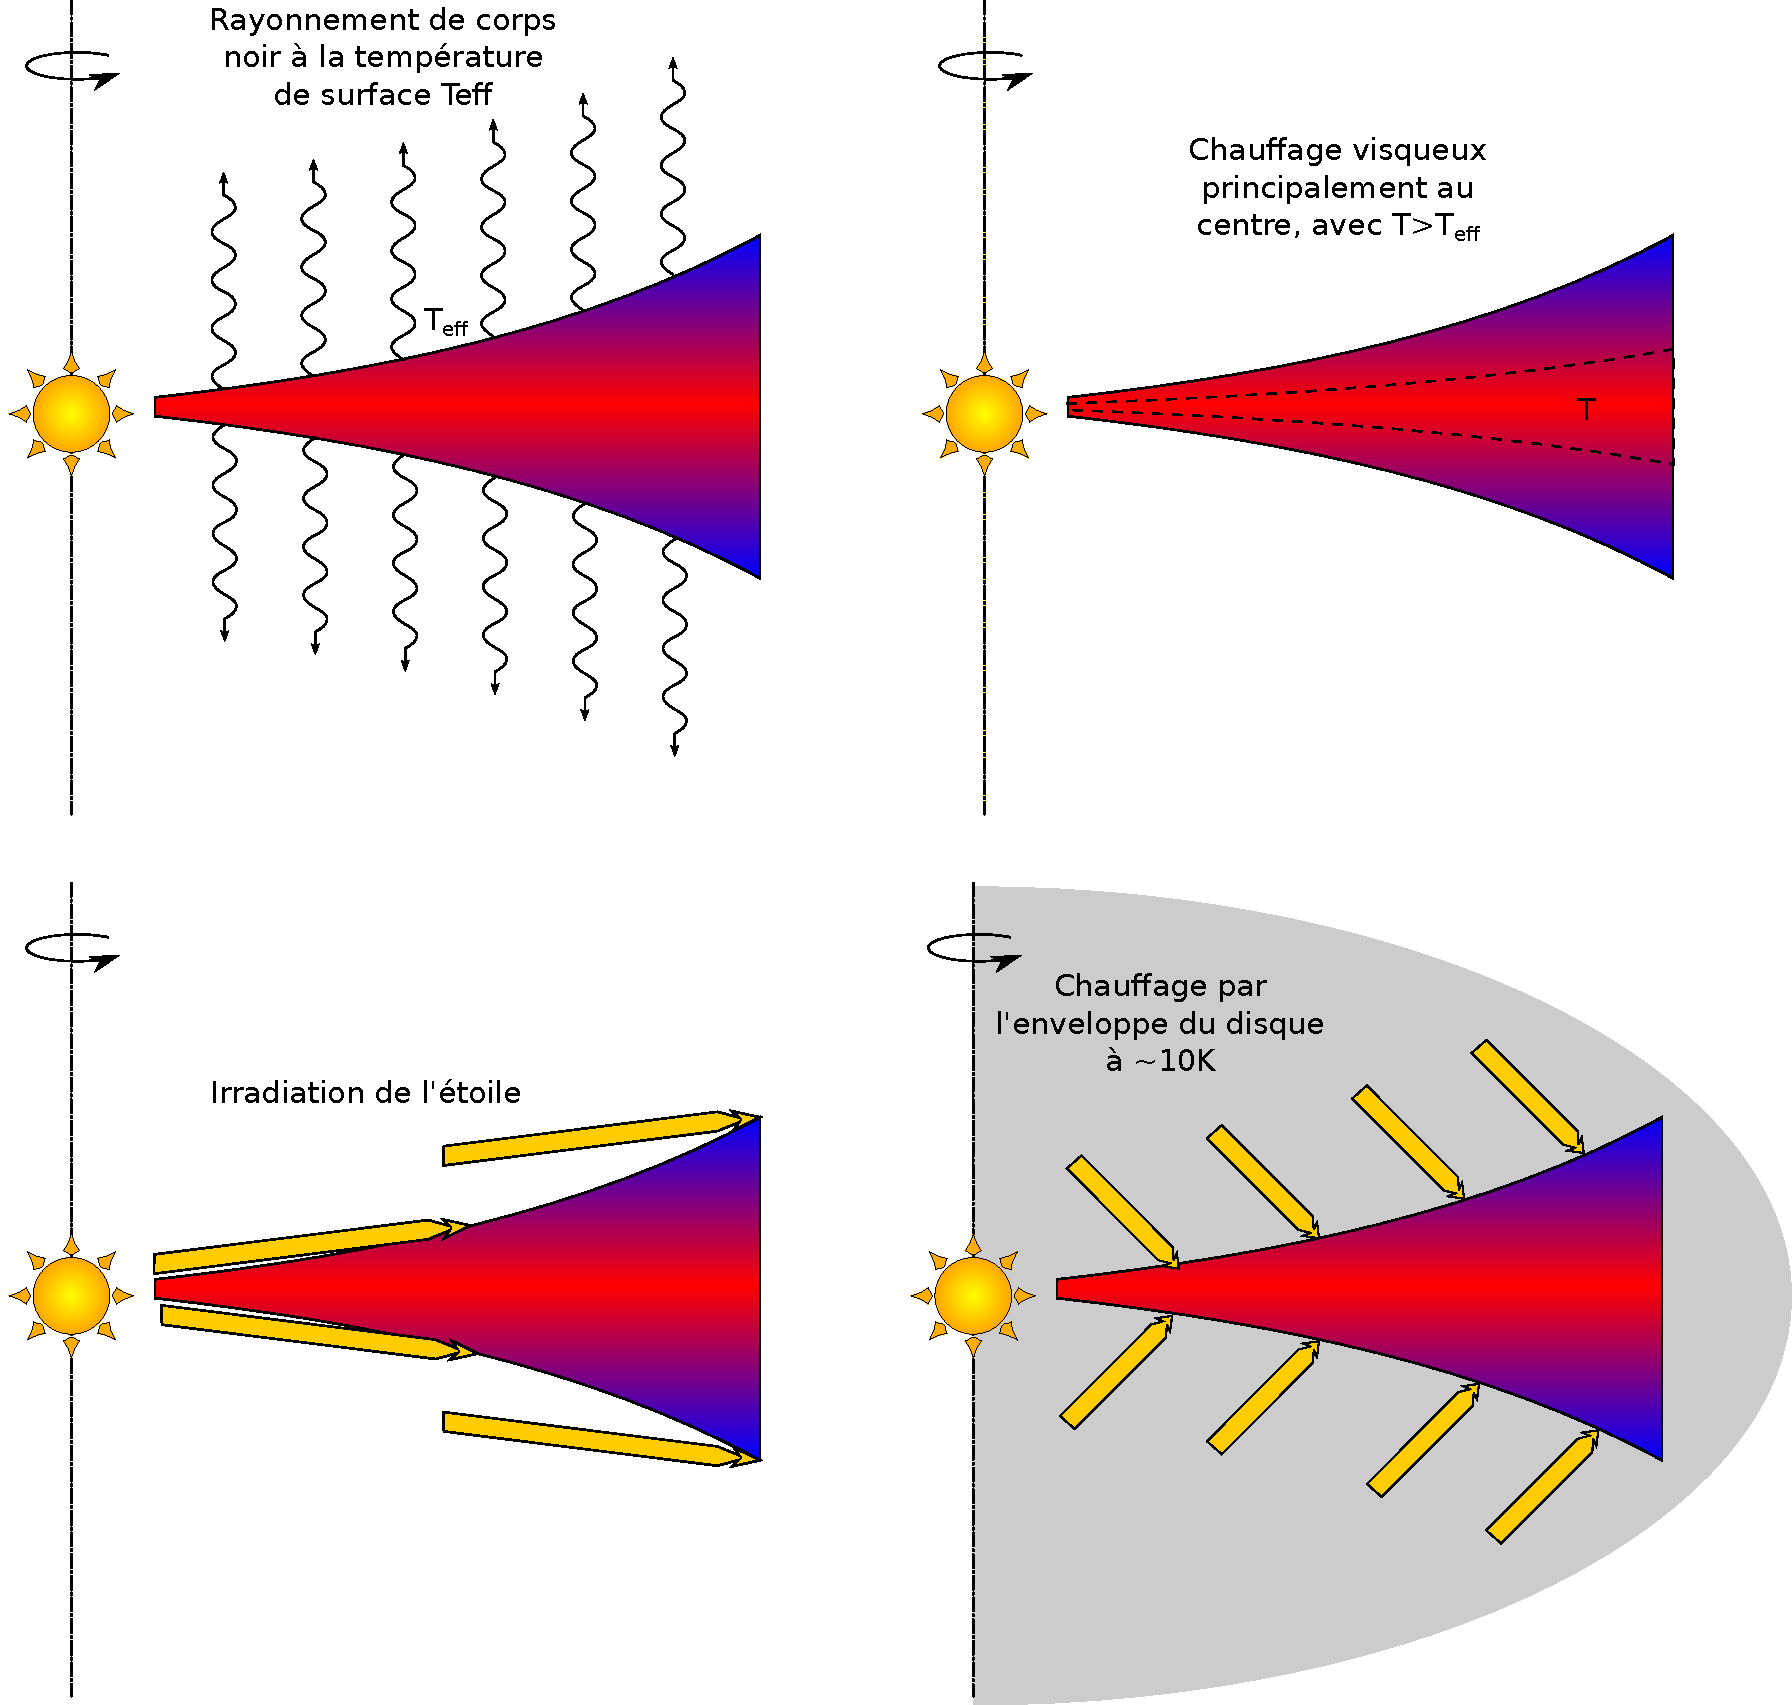
\includegraphics[width=0.45\linewidth]{figure/disk_energy.pdf}
\caption{Représentation du bilan thermique d'un disque}\label{fig:energy_equilibrium}
\end{figure}

\subsubsection{Refroidissement radiatif}
Par toute la surface du disque, qui est à une température $T_\text{eff}$ en surface, on a des pertes par rayonnement : 
\begin{align}
P_\text{cn} &= - 2\sigma T^4
\end{align}
où $\sigma$ est la constante de Stephan. Ces dernières doivent être multiplié par deux, en effet, il y a des pertes par rayonnements des deux cotés du disque à une position donnée. 

\subsubsection{Chauffage par l'enveloppe}
\begin{figure}[htb]
\centering
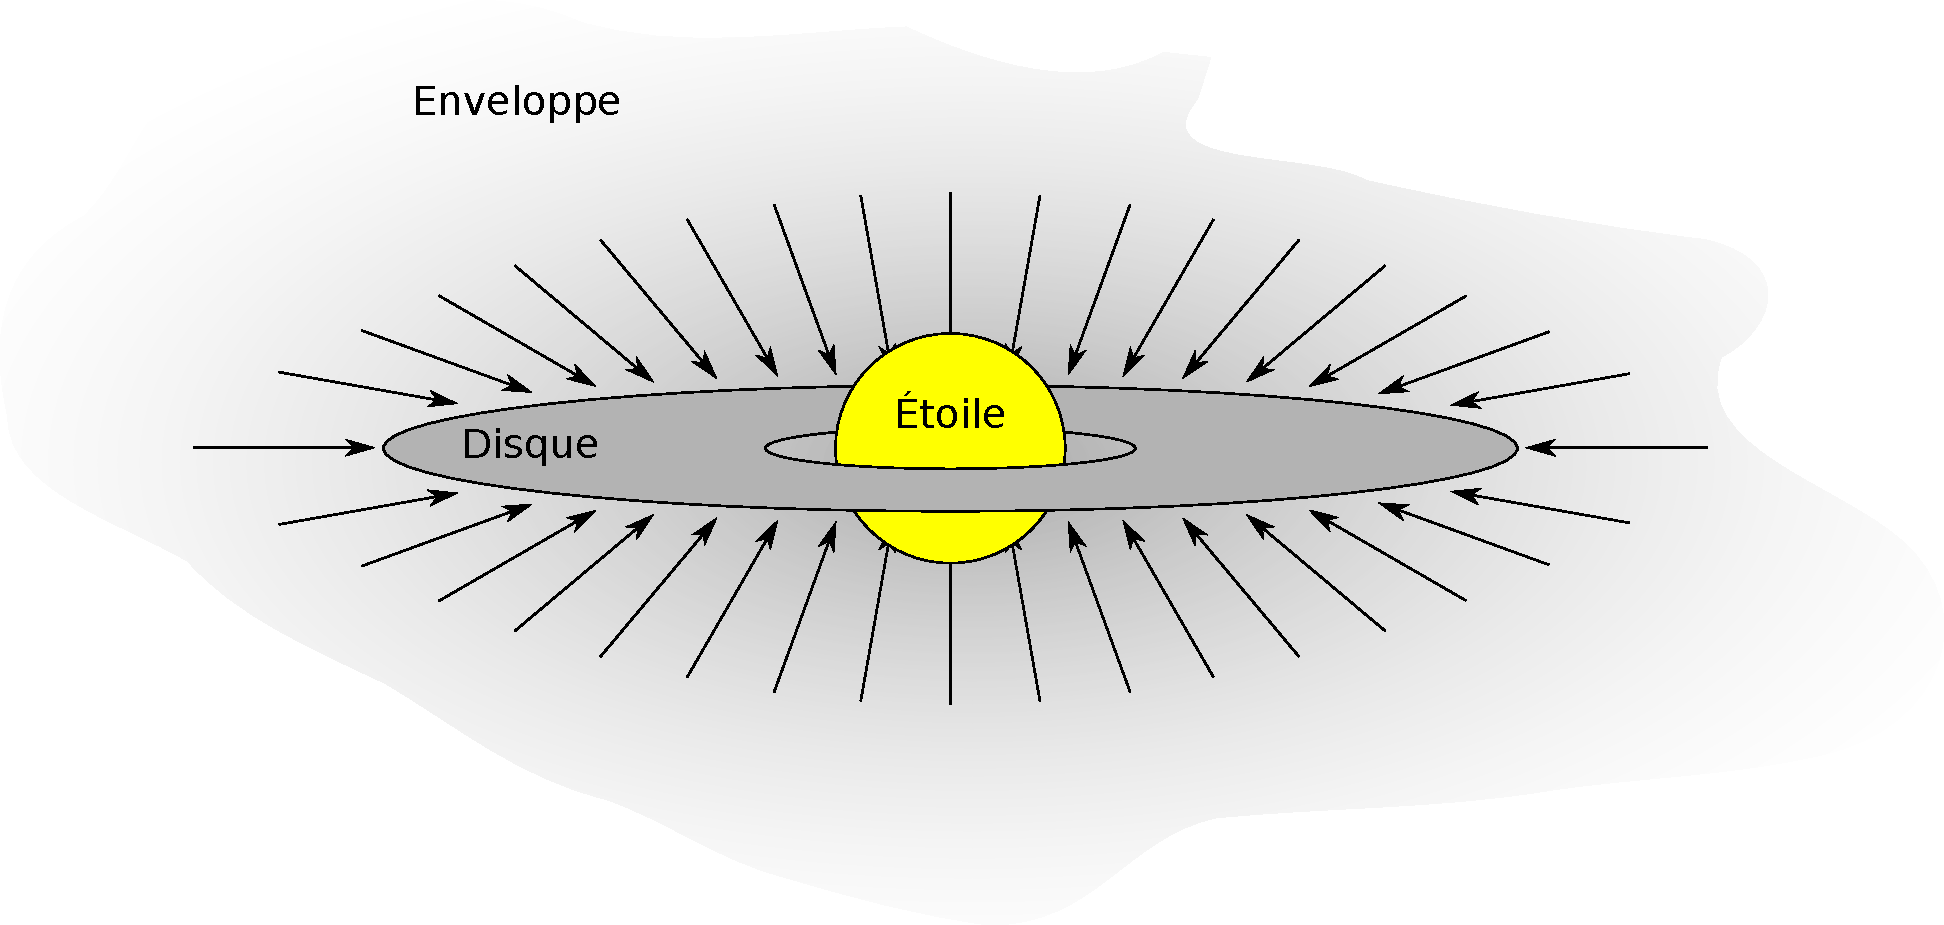
\includegraphics[width=0.45\linewidth]{figure/disk_envelope.pdf}
\caption{Représentation de l'effondrement d'un nuage moléculaire et des différentes parties qui composent le système en effondrement.}\label{fig:envelope}
\end{figure}
L'enveloppe \reffig{fig:envelope} provient de l'effondrement continu du nuage moléculaire. C'est un reste diffus qui alimente continuellement le disque en matière. Mais cette enveloppe, qui possède une température que l'on fixe ici à $T_\text{en} = 10\unit{K}$ contribue aussi au bilan d'énergie du disque en apportant la contribution uniforme suivante :
\begin{align}
C_\text{en} &= 2 \sigma {T_\text{en}}^4
\end{align}

\subsubsection{Chauffage par l'étoile}
La surface du disque reçoit de la lumière de l'étoile centrale. Soit $R_\star$, $L_\star$ respectivement le rayon et la luminosité de l'étoile. Soit $\varepsilon$ l'albédo du disque, que l'on peut typiquement égal à $0.5$. 

Le flux incident est alors \citep[eq. (7)]{menou2004low} : 
\begin{align}
F_\text{irr} &= \frac{L_\star(1-\varepsilon)}{4\pi r^2} \alpha
\end{align}
où $\alpha$ (avec $\alpha\ll 1$ représente l'angle entre les rayons incidents et la surface du disque. 

D'après notamment \cite[eq. (5)]{chiang1997spectral}, cet angle peut être écrit comme : 
\begin{align}
\alpha &= 0.4 \frac{R_\star}{r} + r \dod{}{r}\left(\frac{H}{r}\right)
\end{align}

On note que dans cette expression, le premier terme illustre le fait que l'étoile n'est pas ponctuelle, et que ceci a un effet sur l'irradiation dès que l'on s'approche de cette dernière. Le deuxième terme représente la surface du disque qui intercepte le rayonnement incident, et qui est fonction de la variation d'échelle de hauteur du disque (plus le disque est évasé, et plus la paroi qui intercepte le rayonnement est abrupte). 

Il vient enfin, en exprimant la luminosité de l'étoile en fonction de sa température et de son rayon, l'expression suivante :
\begin{align}
C_\text{irr} &= 2 \sigma {T_\star}^4 \frac{{R_\star}^2}{r^2} (1-\varepsilon) * \left[0.4 \frac{R_\star}{r} + r \dod{}{r}\left(\frac{H}{r}\right)\right]
\end{align}


%non ponctualité de l'étoile : Chiang & Goldreich, 1997, ApJ, 490, 368
%expression de l'angle notammenet : dullemond 2000
%autres expressions : menou & goodman 2004

\subsubsection{Chauffage visqueux}


%TODO parler de la température du disque (et les phénomènes principaux qui ont un effet sur la température, chauffage visqueux, irradiation de l'étoile, irradiation externe. Parler dans cette partie de l'opacité, des transitions et à quoi c'est dû, des modèles had oc pour l'opacité et des incertitudes qui en découlent

%TODO finir ça

\subsection{Taille et représentation des disques}%TODO s'inspirer du 2.1.1 de yann en rajoutant un schéma de disque pour illustrer qu'il faut se méfier des représentations vis à vis de la "réalité"

\begin{figure}[htb]
\centering
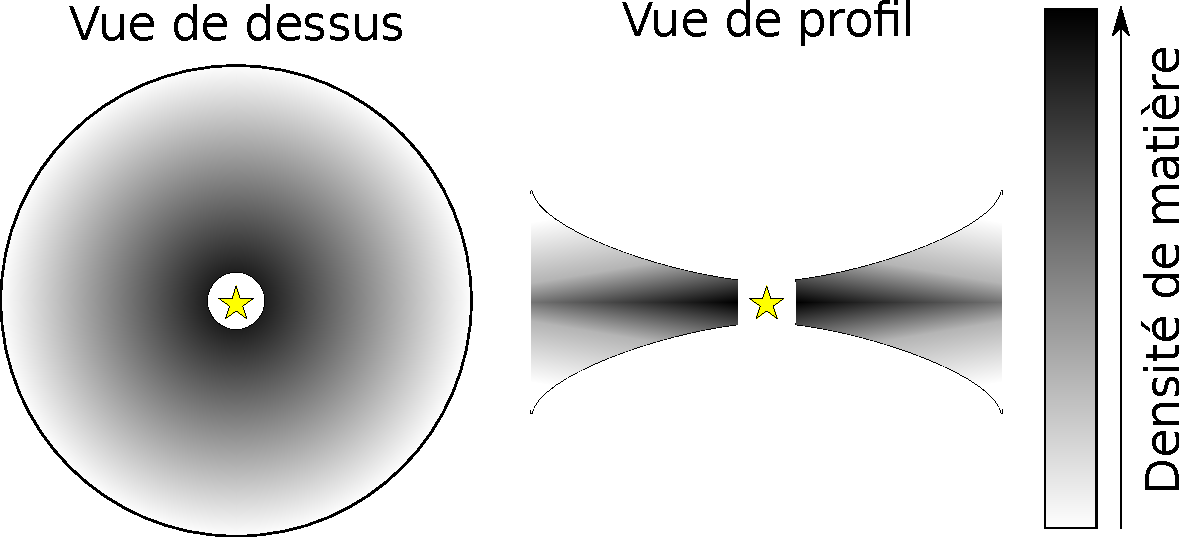
\includegraphics[width=0.45\linewidth]{figure/disk_scheme.pdf}
\caption{Représentation de la répartition radiale et azimutale de matière dans un disque protoplanétaire.}\label{fig:disk_scheme}
\end{figure}

\reffig*{fig:disk_scheme} donne une idée de ce qu'est un disque protoplanétaire. Pour autant, ce n'est qu'une représentation et il est toujours important de garder en tête quelques différences notables entre cette représentation et la réalité physique d'un disque. Quand on parle de disque protoplanétaire, on fait référence à la composante gazeuse, largement majoritaire. Pourtant, bien que minoritaire, la poussière joue un rôle majeur et sa répartition spatiale ne suis pas forcément exactement celle du gaz, ces deux entitées n'ayant pas les mêmes propriétés, elles ne sont pas strictement régies par les mêmes équations.

\bigskip

Tout d'abord, le bord interne est une des parties les plus complexes d'un disque protoplanétaire. Ce bord interne correspond, pour la poussière, à une température de 1500K environ, température au delà de laquelle la partie réfractaire des grains se sublime. 

Le gaz, quant à lui, ne se propage pas non plus jusqu'à la surface de l'étoile en raison du champ magnétique important autour des jeunes étoiles. Le bord interne est ainsi déterminé par le rayon de co-rotation de l'étoile, c'est à dire la distance à laquelle une particule en rotation képlerienne orbite à la vitesse de rotation de l'étoile. Le champ magnétique de l'étoile tournant à la vitesse de rotation de l'étoile, ce rayon de co-rotation correspond ainsi au rayon en dessous duquel le gaz est freiné par le champ magnétique et est rapidement accrété le long des lignes de champ. 

\bigskip

En considérant un système \og étoile + disque\fg isolé, il n'y a pas d'arrêt brutal de la distribution de matière au bord externe qui est donc plus une limitation numérique nécessaire aux simulations qu'autre chose. La réalité est représentée plus fidèlement par une décroissante continue de la matière, difficile à représenter tant pour le bord externe que pour la distribution azimutale du disque. 

Généralement, on considère donc que la taille verticale du disque est égale à une échelle de hauteur (grandeur caractéristique de la décroissance exponentielle verticale de la densité de matière), tandis que la taille radiale du disque dépend de la physique que l'on considère. Dans mon cas j'ai souvent pris un bord externe à 100 AU.


%TODO !!!! Parler de l'équation et parler de manière logique des différents termes et paramètres qui en découlent.

%TODO 
\subsection{Le rôle prépondérant de la poussière}
Le disque est principalement composé de gaz, hydrogène et hélium en majorité. Pour autant, c'est bien la poussière qui est au centre de toutes les attentions, même si cette dernière ne représente qu'1\% de la masse du disque environ.

À cause de la pression quasi inexistante dans le disque en raison des faibles densités, solide et gaz sont les seules phases existantes, il n'y a pas de liquides dans l'espace. La poussière représente la matière solide du disque, en grain plus ou moins fin, allant du nanomètre, micromètre, jusqu'à des tailles planétaires en fin de formation. 

Cette poussière est un composé extrêmement complexe à manipuler. Elle contient différents composés solides en fonction de la température (à certaines températures et densité des composés se volatilisent et d'autres non). La ligne des glaces est une ligne imaginaire au delà de laquelle de la glace d'eau apparait, augmentant de manière drastique la quantité de poussière dans le disque. 

\bigskip

De plus, la poussière est aussi responsable de l'opacité du disque, c'est à dire sa capacité à laisser passer ou non la lumière. À travers l'opacité, la poussière a donc une influence sur la température du disque qui se refroidit plus ou moins efficacement, et qui absorbe le rayonnement stellaire plus ou moins efficacement. 

\subsection{La viscosité du disque} \index{viscosité}% (Franck et al. 1992)
Quand on parle de viscosité $\nu$ dans un disque, ce n'est pas la viscosité moléculaire classique, bien trop faible aux densités rencontrées. On suppose généralement une viscosité due aux turbulences qui est beaucoup plus importante que la viscosité moléculaire, mais qui peut être traitée par les mêmes équations. 

Ceci implique par contre qu'il y ait de l'ionisation. En effet, sans ionisation, il n'y a pas de couplage entre le champ magnétique et la matière, et donc pas de turbulence induite par ce même champ. 

Dans la pratique, il est rare que la viscosité soit calculée de manière cohérente, ce qui serait beaucoup trop couteux en calculs, sans apporter forcément beaucoup plus de précisions étant donné les nombreuses incertitudes sur la poussière, le couplage et le champ magnétique. 

La première hypothèse est de considérer une viscosité constante. Faute de mieux, c'est ce qui semble être le plus évident. On peut, si on veut affiner, utiliser une théorie dite des \gras{disque-alpha}

\subsubsection{Les disques alpha}
On peut introduire un paramètre adimensionné $\alpha$ \citep{shakura1989black}. Dans ce formalisme, plusieurs hypothèses sont faites : 
\begin{itemize}
\item On considère que les turbulences sont sub-soniques.
\item L'échelle des tourbillons des turbulences est plus petite que l'échelle de hauteur du disque
\end{itemize}
Le mécanisme qui a le plus de chance d'être à l'origine de la viscosité alpha est l'\gras{Instabilité Magnéto-Rotationnelle} (MRI). 

\bigskip

En conséquence, on peut définir la viscosité $\nu$ associée aux turbulences comme étant 
\begin{align}
\nu &= \alpha c_s H
\end{align}
où $c_s$ est la vitesse du son et $H$ l'échelle de hauteur du disque. $\alpha$ (avec $\alpha < 1$) est alors un paramètre adimensionné qui permet de définir plus ou moins l'intensité des turbulences, et donc la viscosité qui leur est associée. Une valeur typique d'$\alpha$ se situe entre $10^{-2}$ et $10^{-4}$.

Même si cette prescription simplifie un peu le problème, il semble probable qu'$\alpha$ ne soit pas constant, et dépende de la position dans le disque. On déplace alors le problème, vu que se pose la question des variations d'$\alpha$ dans le disque, notamment la dépendance radiale de ce dernier.

\subsection{Ionisation et dead-zones}\index{ionisation}\index{dead zone}
Pour qu'une instabilité magnéto rotationnelle ait lieu, c'est à dire qu'il y ait un couplage entre le champ magnétique et les mouvements du disque, il faut qu'une partie au moins du disque soit ionisé. Dans ces régions ionisées, on pourra alors avoir transport du moment angulaire via la viscosité due au champ magnétique (et turbulences engendrées). 

Or, comment ioniser? Que ce soit le rayonnement X de l'étoile centrale, des rayons cosmiques ou l'ionisation thermique, il n'est pas si évident que ça de se représenter l'ionisation totale du disque de gaz. Il est donc probable que certaines zones du disques ne soient pas ionisés, et donc que le transport du moment angulaire s'y fasse peu ou pas du tout. Ces zones, appelées \index{dead zone}, sont donc des zones sans viscosité magnétique. %TODO compléter la partie dead zone

\begin{figure}[htb]
\centering
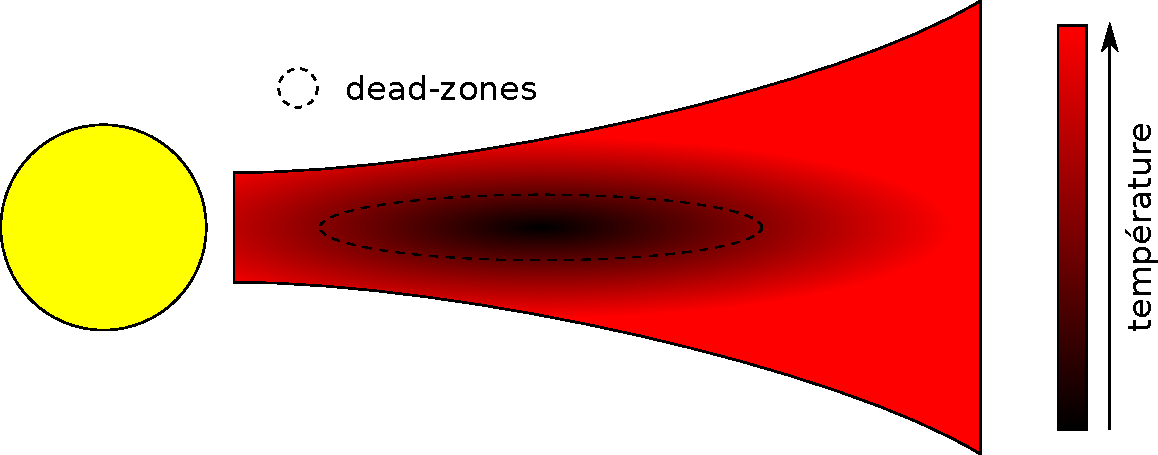
\includegraphics[width=0.7\linewidth]{figure/dead_zones.pdf}
\caption{Représentation d'un disque à couches (layered disk). L'ionisation d'une zone est déterminé par sa température. Ainsi, les zones internes à température plus faible ne sont pas ionisés et n'ont donc pas de viscosité dûes aux turbulences magnétique (MRI). Les régions externes ne sont pas des zones mortes parce qu'elles peuvent être sujettes à des ionisations non thermiques en raison de leur densité plus faible. À distance intermédiaire, le disque est trop froid pour de l'ionisation thermique, et trop dense pour de l'ionisation non thermique.}\label{fig:dead_zones}
\end{figure}


%TODO j'en suis à la page 158 du .pdf ``accretion processes in star formation''

\subsection{Profil de densité}
%TODO 

\subsection{Les bords du disque}
%TODO parler des bords du disque et de tous les problèmes que ça pose

\section{Interaction disque-planète}
\subsection{Migration planétaire}
%TODO 
\subsubsection{Type I}\index{migration!type I}
Ce type de migration ne concerne que les planètes de faible masse (de l'ordre de $10M_{\oplus}$)pour lesquelles l'interaction de marée entre la planète et le disque a une réponse linéaire (Le profil de densité surfacique reste quasiment le même). Ces planètes, qui ne creusent pas de sillon (gap) dans le disque de gaz, vont migrer vers l'intérieur.

\begin{remarque}
Pour plus de détails, se référer au chapitre 9, page 188--191 de \cite{barnes2010formation} ou \cite{ward1997protoplanet} pour l'article original.
\end{remarque}

La présence d'une planète dans un disque de gaz entraine la création d'ondes de densités aux \gras[résonnance!de Lindblad]{résonances de Lindblad} \citep{goldreich1979excitation}. Le couplage gravitationnel entre les ondes de densité et la planète qui les crées abouti à un \gras{couple} qui agit sur la planète.

Lors de la création d'ondes de densité par une planète dans un disque, il se forme un déséquilibre naturel entre les couples agissant sur les disques internes et externes. La position des résonances de Lindblad externes tend à être plus proche de la planète que ne l'est celle des résonances internes.


%TODO 
\subsubsection{Type II}\index{migration!type II}
Quand une planète dans un disque devient suffisamment massive, la réponse du disque n'est plus linéaire, et des ondes de densité induites par la planète forment des chocs non loin de là où elles sont émises. La répulsion entre le disque et la planète devient si forte qu'une cavité annulaire se forme autour de l'orbite de la planète, creusant le disque de gaz.

Une fois que la cavité est formée, la planète est dite en migration de \emph{type II} : son orbite agit alors essentiellement comme une barrière entre les deux parties du disque de gaz, \emph{interne} et \emph{externe}. Du gaz peut parfois sauter le gap, ou être accrêté par la planète mais cette dernière voit son mouvement régit par le disque de gaz, se retrouvant entraînée par la migration de celui-ci.

Compte tenu que la planète a une masse de l'ordre de\footnote{Quand la masse de la planète devient supérieure à la masse du disque local, l'inertie de celle-ci devient importante afin de déterminer son taux de migration} la masse du disque local (avec lequel elle interagit), la migration se passe sur des temps de l'ordre du \gras{temps visqueux} du disque.

\begin{remarque}
Pour plus de détails, se référer au chapitre 9, page 191--192 de \cite{barnes2010formation} ou \cite{lin1986tidal} pour des détails sur les planètes capables de former un sillon dans le disque de gaz.
\end{remarque}
%TODO 
\subsubsection{Type III}\index{migration!type III}

%TODO faire ya page 192 du bouquin de barnes un truc sur \c ca, même si c'est pas explicite dans le titre.

\begin{remarque}
Pour plus de détails, se référer au chapitre 9, page 192--193 de \cite{barnes2010formation} ou \cite{masset2003runaway}.
\end{remarque}
%TODO 

\subsection{L'amortissement de l'excentricité}%circularisation
%TODO parler des autres phénomènes importants dans le disque, comme l'amortissement de l'excentricité

\subsection{L'amortissement de l'inclinaison}%coplanarisation
%TODO parler de l'amortissement de l'inclinaison, 

\subsection{L'accrétion du gaz}\label{sec:accretion_coeur}
Dans le modèle d'\gras[modèle!accrétion de c\oe ur]{accrétion de c\oe ur}, les planètes géantes sont d'abord des c\oe urs rocheux qui grossissent jusqu'à atteindre une masse critique de l'ordre de $15 M_{\oplus}$. Une fois cette masse atteinte, le c\oe ur commence à accréter rapidement du gaz jusqu'à former une géante gazeuse.

Ceci implique que la formation des planètes géantes doive se passer avant que le disque de gaz ne se dissipe (ce qui intervient au bout de $10^7$ ans environ).

Les noyaux de ces planètes sont supposés se former au delà de la ligne des glaces (limite radiale virtuelle au delà de laquelle on peut trouver de l'eau sous forme solide ; autour de $4\unit{ua}$). En effet, au delà de cette limite, la quantité de matière solide augmente, et donc le taux d'accrétion augmente aussi.

\begin{attention}
La formation des embryons de planètes géantes n'est toujours pas clair. On ne sait pas vraiment s'il y a une zone privilégiée ou non, la limite virtuelle de la ligne des glaces pourrait ne pas être valable, la glace ne rajoutant qu'environ 50\% de masse en plus.\index{ligne des glaces}\index{snowline|see{ligne des glaces}}

À noter qu'il n'y a pas de pression et donc pas de liquide dans l'espace, juste du gaz ou du solide.
\end{attention}

\bigskip

Pour une simulation donnée, si on augmente le taux d'accrétion de la planète, celle-ci sera plus massive, et aura donc une inertie plus grande. Elle mettra donc plus de temps à migrer\index{migration} par migration Type II car son inertie s'y opposera. D'un autre coté, si la planète n'a pas encore créé de gap, la migration de Type I est plus rapide à mesure que la masse augmente. 

%TODO parler de l'accrétion, et du fait que ça va créer des planètes géantes notamment

\subsection{Récapitulatif des interactions dans le code N-corps}
%TODO parler du fait que je ne prend pas en compte l'accrétion de gaz, les gaps, 